\documentclass[utf8,xcolor=table, page number]{earlywinter}

\usepackage[T1]{fontenc}
\usepackage[frenchb]{babel}
\usepackage{graphicx}

\begin{document}
\title{Edge Cloud Computing}
\subtitle{Bringing the Cloud to the Edge}
\author{Aurèle BARRIÈRE & Solène MIRLIAZ}

\begin{frame}[plain]
  \titlepage%
\end{frame}

% ----------------
% - Introduction -
% ----------------
\section{Introduction}
\begin{frame}
	\frametitle{\secname}
  \framesubtitle{Cloud model}
  \begin{center}
    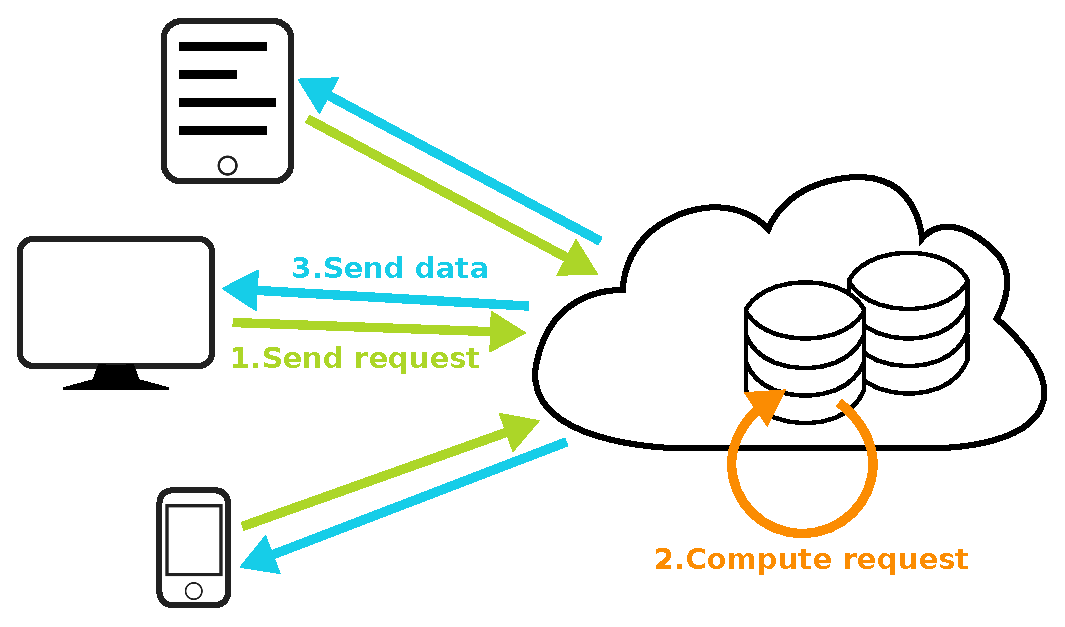
\includegraphics[width=0.7\linewidth]{cloud.eps}
  \end{center}
  \begin{block}{Principle}
    Optimize ressource usage
  \end{block}
\end{frame}
\begin{frame}
	\frametitle{\secname}
  \framesubtitle{Cloud limits}
  \begin{minipage}[l]{0.6\linewidth}
  \begin{block}{Internet of things}
    Growth of the number of connected objects and sensors that generate data.
    The end nodes are evolving from consumers to producers.
    
    Estimated produced data by 2019: \emph{500 zettabytes} {\tiny (estimate by Cisco Global Cloud Index)}.
  \end{block}
  \end{minipage}
  \begin{minipage}[l]{0.3\linewidth}
    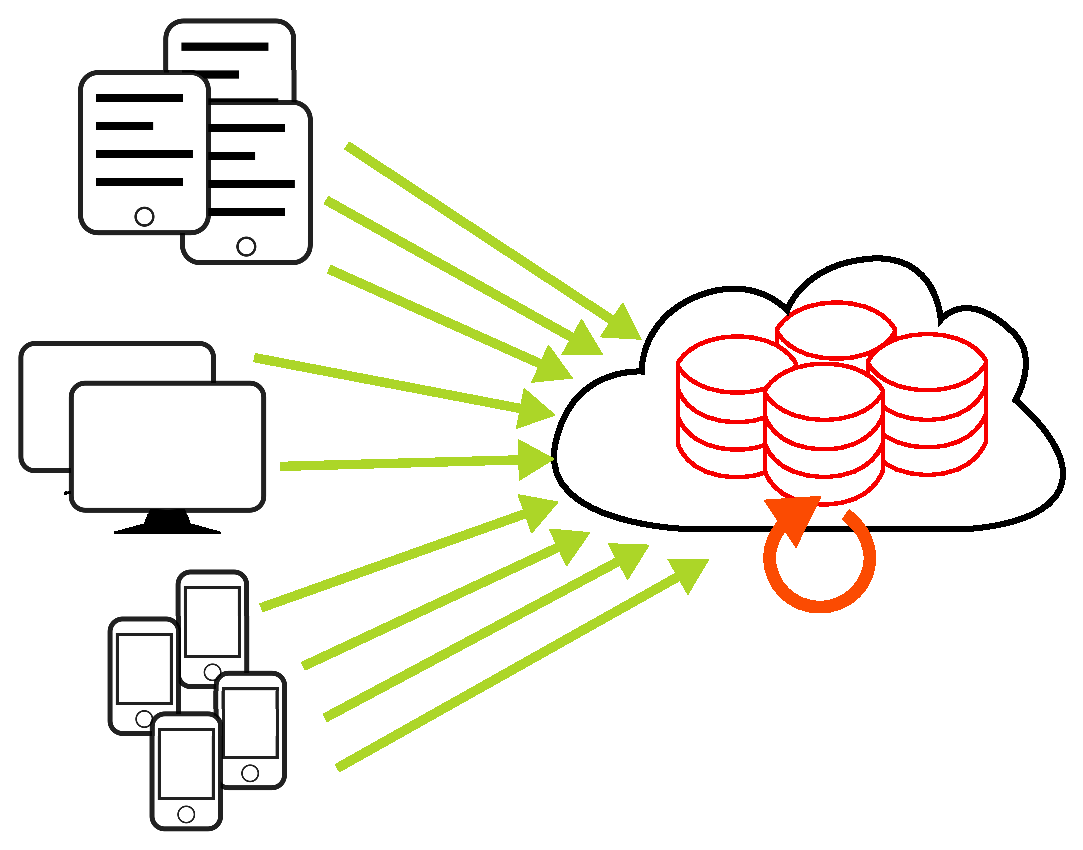
\includegraphics[width=1.5\linewidth]{cloudlimits.eps}
  \end{minipage}
	\begin{alertblock}{Limits of the clouds}
          \begin{itemize}
            \item The network can't handle that much.\\
              Estimated IP traffic by 2019: 10.4 zettabytes.
            \item The Cloud's computation power can't handle that much.
            \item For many uses, the Cloud introduces too much latency.
            \item Centralization brings privacy issues.
          \end{itemize}
	\end{alertblock}
\end{frame}
\begin{frame}
	\frametitle{\secname}
  \framesubtitle{Fog model}
  \begin{center}
    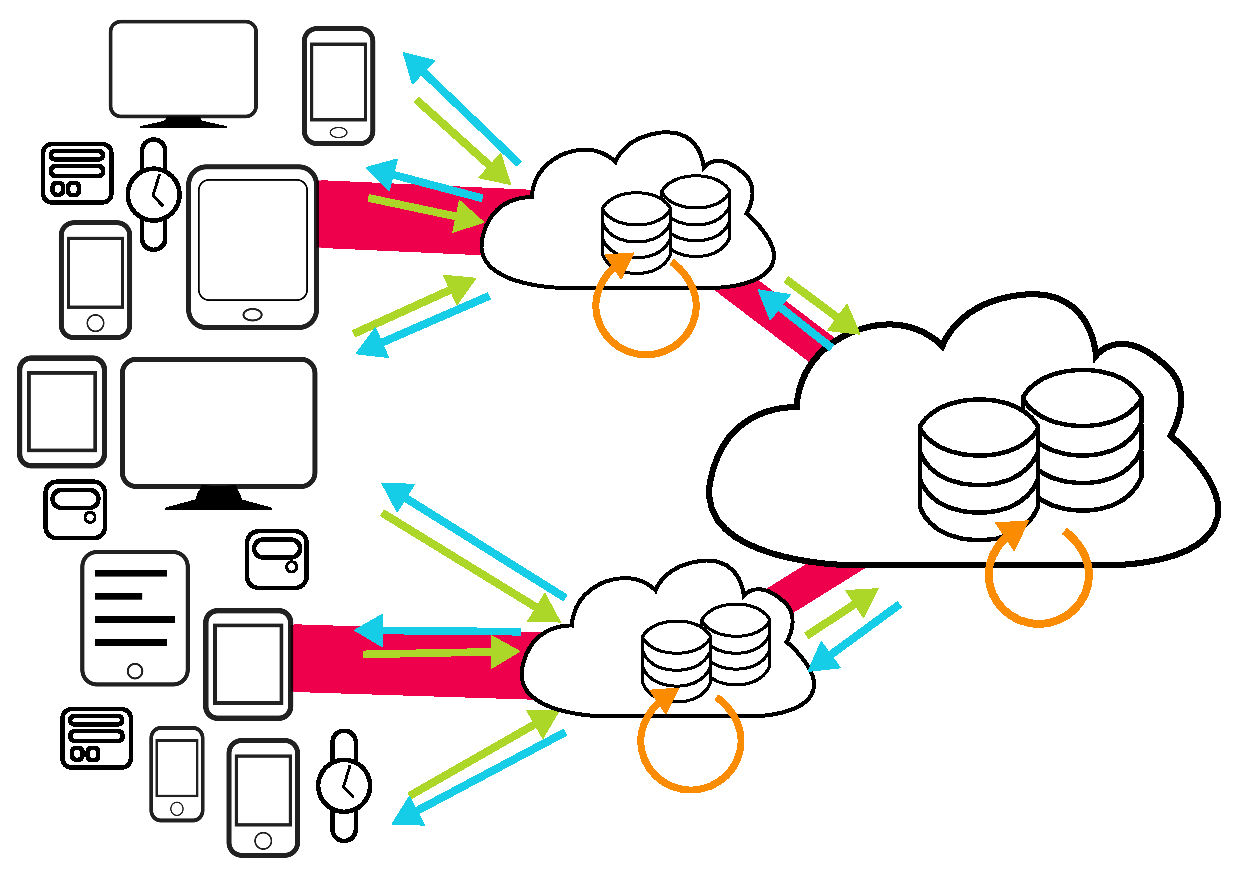
\includegraphics[width=0.7\linewidth]{fog.eps}
  \end{center}
  \begin{block}{Principle}
    More little clouds, closer to the devices $\to$ Spread the ressources
  \end{block}
\end{frame}
\begin{frame}
	\frametitle{\secname}
  \framesubtitle{Edge model}
  \begin{center}
    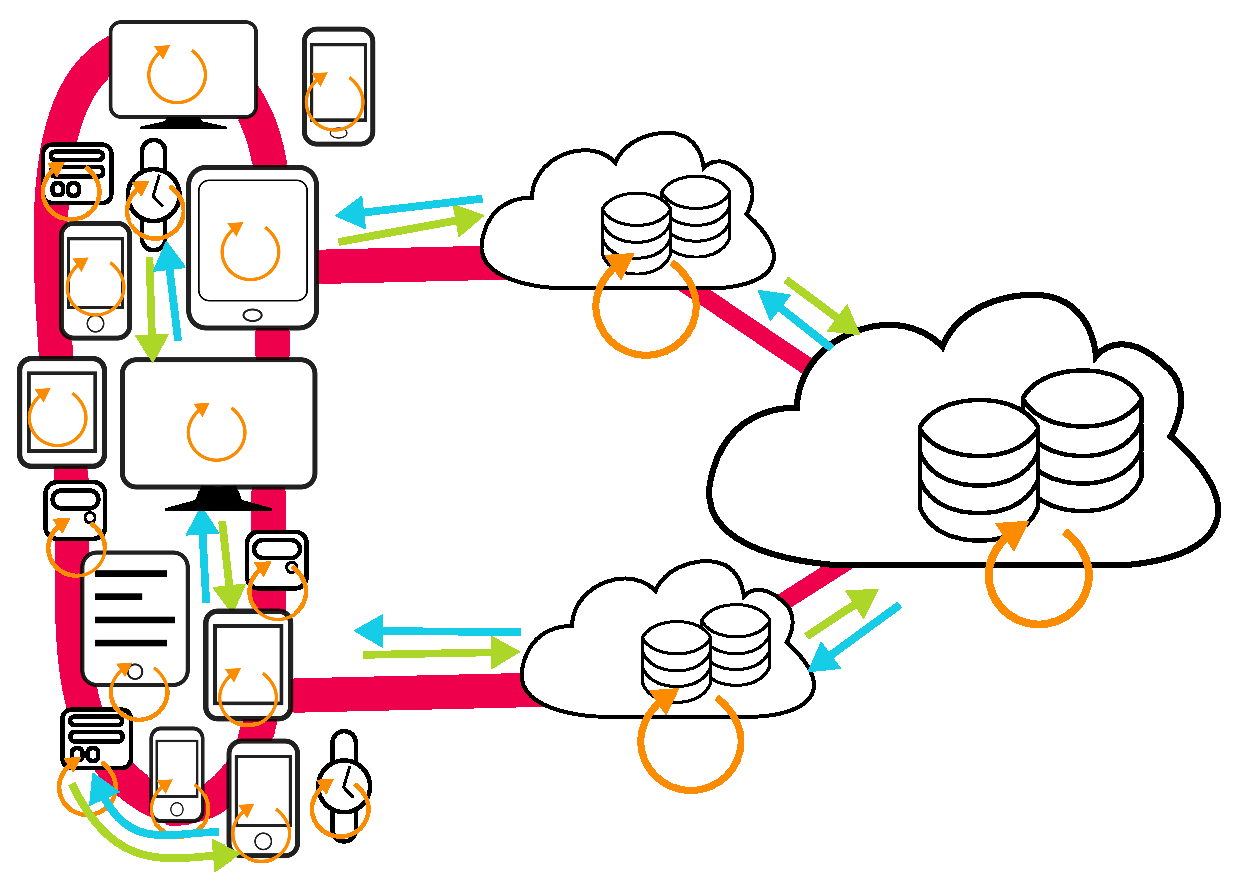
\includegraphics[width=0.6\linewidth]{edge.eps}
  \end{center}
  \begin{block}{Principle}
    More computation done on the devices, more communication between close devices.
  \end{block}
\end{frame}

  \begin{frame}
    \frametitle{Table of contents}
    \tableofcontents[]
  \end{frame}
  
  
\section{Edge computing challenges}
\subsection{Bringing the cloud to the Edge: an hybrid system} %I'm not sure this is a good phrasing. maybe some of the papers we read would disagree
\begin{frame}
  \frametitle{Edge computing}
  \framesubtitle{Principle}

  \begin{block}{Computing in the Edge}
    Increase in the nodes' computing power (smartphones, embedded devices).
  \end{block}
   We want to put computing at the proximity of data sources: at the Edge.

   It could either be in the nodes themselves, or in smaller edge servers. We can use already existing CDNs to put such servers.
  
   \begin{exampleblock}{Example: Smart Home}
     In a smart home, the data produced by every sensor could be consumed directly without sending it to a datacenter.
   \end{exampleblock}

\end{frame}

\begin{frame}
  \frametitle{Edge-Cloud computing}
  \framesubtitle{An hybrid system}

%  \begin{figure}
%    \center
%    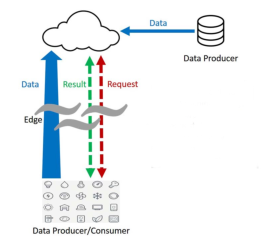
\includegraphics[scale=0.5]{edge.png}  %I'm not a big fan of this graphic. might have to change it.
%  \end{figure}
%
  Keep using the Cloud (core), but add computation at the Edge.
  The Cloud keeps providing global services, but edge servers can compute with lower latency.

  We can then use advantages from both the Cloud and the Edge.
  
  \begin{exampleblock}{Example: Online Shopping}
    We want fast browsing, although synchonization with a global server is needed.
  \end{exampleblock}

  In this example, cloud synchronization could be done in background.
  
\end{frame}

\begin{frame}
\frametitle{Edge-Cloud Computing}
\framesubtitle{Overview}

ADD SCHEMA

\end{frame}

\subsection{Challenges}

% the challenges and research interests are almost the same to me

\begin{frame}
  \frametitle{Challenges}
  \framesubtitle{Energy}
  
  Mobile device with low battery
  
\end{frame}
\begin{frame}
  \frametitle{Challenges}
  \framesubtitle{Computing power}
  
  Increasing
  
\end{frame}
\begin{frame}
  \frametitle{Challenges}
  \framesubtitle{Mobility}
  
  Mobile things. Failure-tolerence must be high.
  
  Where to put the service in the edge?
  
\end{frame}
\begin{frame}
  \frametitle{Challenges}
  \framesubtitle{Heterogenity}
  
  Of the network and things' abilities.
  
	\begin{example}
		Cellphone, Oven, radio, heater, computer, etc.
	\end{example}
  
  Of the programming languages used by each.  
  
  Of the applications
	\begin{example}
		High CPU need, high memory need, quick communication, etc.
	\end{example}
  
\end{frame}

% \section{Current research studies}
% \subsection{Architecture}
% \begin{frame}
%   \frametitle{Current Research}
%   \framesubtitle{Architecture}
% 
%   Edge-cloud computing requires new connections between users, edge nodes, edge networks, datacenters...
% 
%   
% 
% \end{frame}
% \subsection{Workload Distribution}
% \begin{frame}
%   \frametitle{Current Research}
%   \framesubtitle{Workload Distribution}
% \end{frame}
% \subsection{Problem Identification and Heuristics}
% \begin{frame}
%   \frametitle{Current Research}
%   \framesubtitle{Problem Identification and Heuristics}
%   \begin{exampleblock}{On-demand gaming coverage} % [4]
%     We need a low-latency service that can satisfy the most people.\\
%     We need heuristics for edge servers deployment.
%   \end{exampleblock}
% \end{frame}
% \subsection{Programmability}
% \begin{frame}
%   \frametitle{Current Research}
%   \framesubtitle{Programmability}
% \end{frame}
% \subsection{Naming}
% \begin{frame}
%   \frametitle{Current Research}
%   \framesubtitle{Naming}
% \end{frame}
% 
% \section{Case example: a traffic light}
% \begin{frame}
%   \frametitle{Case Example}
%   \framesubtitle{Smart Traffic Light}
% \end{frame}


\section{Use Cases}

\begin{frame}
  \frametitle{Use Cases}
  \framesubtitle{And Research interests}

  \begin{block}{}
    In which cases is Edge-Cloud Computing more efficient than Cloud-only or Edge-only approaches?
  \end{block}

\end{frame}

\subsection{Exploiting locality}
\begin{frame}
  \frametitle{\secname}
  \framesubtitle{\subsecname}

  \begin{exampleblock}{Indoor 3D localization}
    Smartphones gather data from the camera and accelerometer.\\
    Computation can be done in the edge (latency) or in the core (reliability).
  \end{exampleblock}

  \begin{center}
  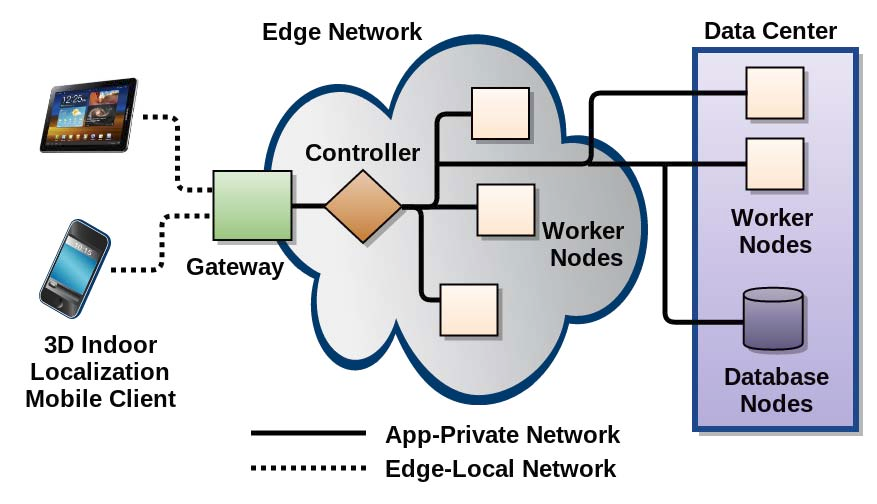
\includegraphics[scale=0.2]{indoor}
  \end{center}

  

\end{frame}

\subsection{Reducing the network usage}
\begin{frame}
  \frametitle{\secname}
  \framesubtitle{\subsecname}

  With the Internet of Things, and in general the huge increase in produced data, we can't assume that our network could handle that much.

  \begin{exampleblock}{Smart Cities, Smart Homes}
    A lot of the produced data could be consumed locally. We could still use centralization (EXAMPLE)
  \end{exampleblock}
  
\end{frame}


\subsection{Analyzing data at different time scales}
\begin{frame}
  \frametitle{\secname}
  \framesubtitle{\subsecname}

  \begin{exampleblock}{Online Shopping}
    We need a responsive user interface. We want centralized data.
  \end{exampleblock}

  \begin{exampleblock}{Smart Traffic Light System}
    We want centralized data to regulate traffic on a large scale.\\
    We want low-latency response when dealing with local events (EXAMPLE).
  \end{exampleblock}
  
\end{frame}

\subsection{Reduce the workload in the Cloud}
\begin{frame}
  \frametitle{\secname}
  \framesubtitle{\subsecname}

  \begin{exampleblock}{Video Surveillance}
    For instance, to find a missing child, we need fast video analysis.\\
    Exploits locality.
  \end{exampleblock}

  \begin{alertblock}{Programmability}
    If we want our application to run on nodes, edge servers, could datacenters...\\
    We need a suitable API.
  \end{alertblock}

  \begin{alertblock}{Workload Distribution}
    We are using heterogeneous and mobile ressources for computation.
  \end{alertblock}
  
\end{frame}


\subsection{Better coverage for low-latency applications}
\begin{frame}
  \frametitle{\secname}
  \framesubtitle{\subsecname}

  \begin{exampleblock}{On-demand Gaming}
    The service needs low-latency. Cloud servers could only cover less than 75\% of the US population.
  \end{exampleblock}

  \begin{alertblock}{Heuristics for a better coverage}
    We need the most efficient way to put edge servers.
  \end{alertblock}
  
\end{frame}



\begin{frame}{Other Research studies} % I don't really like this name. any suggestion?
  
  \begin{alertblock}{Privacy}
    Some data cannot be sent to anyone (Electronic Medical Records).
  \end{alertblock}

  \begin{alertblock}{Naming Conventions}
    IP protocol isn't suited for the mobility of end nodes devices.
  \end{alertblock}

  % WARNING: I should read more about these two issues. I don't want to say anything stupid
  
\end{frame}



\section{Conclusion}

\begin{frame}
  \frametitle{Conclusion}

  \begin{block}{An hybrid system is needed}
    For some applications, neither cloud-only nor edge-only systems are sufficient.
  \end{block}
  
  \begin{alertblock}{Not a perfect solution}
    In the case of coverage, any reasonnable number of edge servers still let some users without service for now.
  \end{alertblock}
  
  \begin{alertblock}{There's still a lot of work left}
    \begin{itemize}
      \item Lots of open issues
      \item No economical model
    \end{itemize}
  \end{alertblock}

  
\end{frame}


\begin{frame}{When should we use Edge-Cloud Computing?}
% where should we put this?
\begin{itemize}
\item When we need centralized data and low latency (online shopping)
\item When communication from the edge to the core is the bottleneck (Fast video analysis, smart home, smart city)
\item When we can reduce the time of computation by spreading it on the Edge (Video surveillance, missing child)
\item When locality is involved (wind farm, smart city)
\item When some data cannot be shared publicly (hospitals)
\item When some data needs to be stored locally (3D indoor localization)
\item When we want a better coverage for low-latency services (on-demand gaming and multimedia)
\item When we need to analyze data at different time scales (Smart Traffic Light System, wind farm). 
\end{itemize}
\end{frame}


\end{document}
